\chapter{Supplementary Material}

\section{Material from original PGExplainer}
\label{sec:PGE_material}
This section contains the reprinted pseudocode by Luo et al. \cite{luo2020parameterized} in algorithms \ref{alg:node-alg} and \ref{alg:graph-alg}, as well as the accuracies achieved by their used target models in Table \ref{tab:compact-accuracy}.

\begin{algorithm}
    \caption{Training Algorithm for Explaining Node Classification from \cite{luo2020parameterized}.}
    \label{alg:node-alg}
    \begin{algorithmic}[1]
    \REQUIRE Input graph $G_o = (\mathcal{V}, \mathcal{E})$, node features $X$, node labels $Y$, set of instances to be explained $\mathcal{I}$, trained GNN model: $\text{GNNE}_{\Phi_0}(\cdot)$ and $\text{GNNC}_{\Phi_1}(\cdot)$, parameterized explainer MLP $\Psi$.
    \FOR{each node $i \in \mathcal{I}$}
        \STATE $G^{(i)}_o \leftarrow$ extract the computation graph for node $i$.
        \STATE $Z^{(i)} \leftarrow \text{GNNE}_{\Phi_0}(G^{(i)}_o, X)$.
        \STATE $Y^{(i)} \leftarrow \text{GNNC}_{\Phi_1}(Z^{(i)})$.
    \ENDFOR
    \FOR{each epoch}
        \FOR{each node $i \in \mathcal{I}$}
            \STATE $\Omega \leftarrow$ latent variables calculated with (10).
            \FOR{$k \leftarrow 1$ to $K$}
                \STATE $G^{(i,k)}_s \leftarrow$ sampled from (4).
                \STATE $\hat{Y}^{(i,k)}_s \leftarrow \text{GNNC}_{\Phi_1}(\text{GNNE}_{\Phi_0}(G^{(i,k)}_s, X))$.
            \ENDFOR
        \ENDFOR
        \STATE Compute loss with (9).
        \STATE Update parameters $\Psi$ with backpropagation.
    \ENDFOR
    \end{algorithmic}
    \end{algorithm}
    
    \vspace{0.5cm}
    
    \begin{algorithm}
    \caption{Training Algorithm for Explaining Graph Classification from \cite{luo2020parameterized}.}
    \label{alg:graph-alg}
    \begin{algorithmic}[1]
    \REQUIRE A set of input graphs with $i$-th graph represented by $G^{(i)}_o$, node features $X^{(i)}$, label $Y^{(i)}$, trained GNN model: $\text{GNNE}_{\Phi_0}(\cdot)$ and $\text{GNNC}_{\Phi_1}(\cdot)$, parameterized explainer MLP $\Psi$.
    \FOR{each graph $G^{(i)}_o$}
        \STATE $Z^{(i)} \leftarrow \text{GNNE}_{\Phi_0}(G^{(i)}_o, X^{(i)})$.
        \STATE $Y^{(i)} \leftarrow \text{GNNC}_{\Phi_1}(Z^{(i)})$.
    \ENDFOR
    \FOR{each epoch}
        \FOR{each graph $G^{(i)}_o$}
            \STATE $\Omega \leftarrow$ latent variables calculated with (11).
            \FOR{$k \leftarrow 1$ to $K$}
                \STATE $G^{(i,k)}_s \leftarrow$ sampled from (4).
                \STATE $\hat{Y}^{(i,k)}_s \leftarrow \text{GNNC}_{\Phi_1}(\text{GNNE}_{\Phi_0}(G^{(i,k)}_s, X^{(i)}))$.
            \ENDFOR
        \ENDFOR
        \STATE Compute loss with (9).
        \STATE Update parameters $\Psi$ with backpropagation.
    \ENDFOR
    \end{algorithmic}
\end{algorithm}

\begin{table}[h]
    \centering
    \scriptsize
    \begin{tabularx}{\linewidth}{l|X X X X|X X}
    \hline
    \textbf{Accuracy} & \textbf{BA-Shapes} & \textbf{BA-Community} & \textbf{Tree-Cycles} & \textbf{Tree-Grid} & \textbf{BA-2Motif} & \textbf{MUTAG} \\
    \hline
    \textbf{Training}   & 0.98 & 0.99 & 0.99 & 0.92 & 1.00 & 0.87 \\
    \textbf{Validation} & 1.00 & 0.88 & 1.00 & 0.94 & 1.00 & 0.89 \\
    \textbf{Testing}    & 0.97 & 0.93 & 0.99 & 0.94 & 1.00 & 0.87 \\
    \hline
    \end{tabularx}
    \caption[Accuracies of original GNN downstream task]{Compact accuracy table for Node and Graph Classification. Reprinted from \cite{luo2020parameterized}.}
    \label{tab:compact-accuracy}
\end{table}


\section{Data visualization}
\label{sec:data_vis}

\begin{figure}[H]
    \centering
    \begin{subfigure}[b]{0.4\textwidth}
        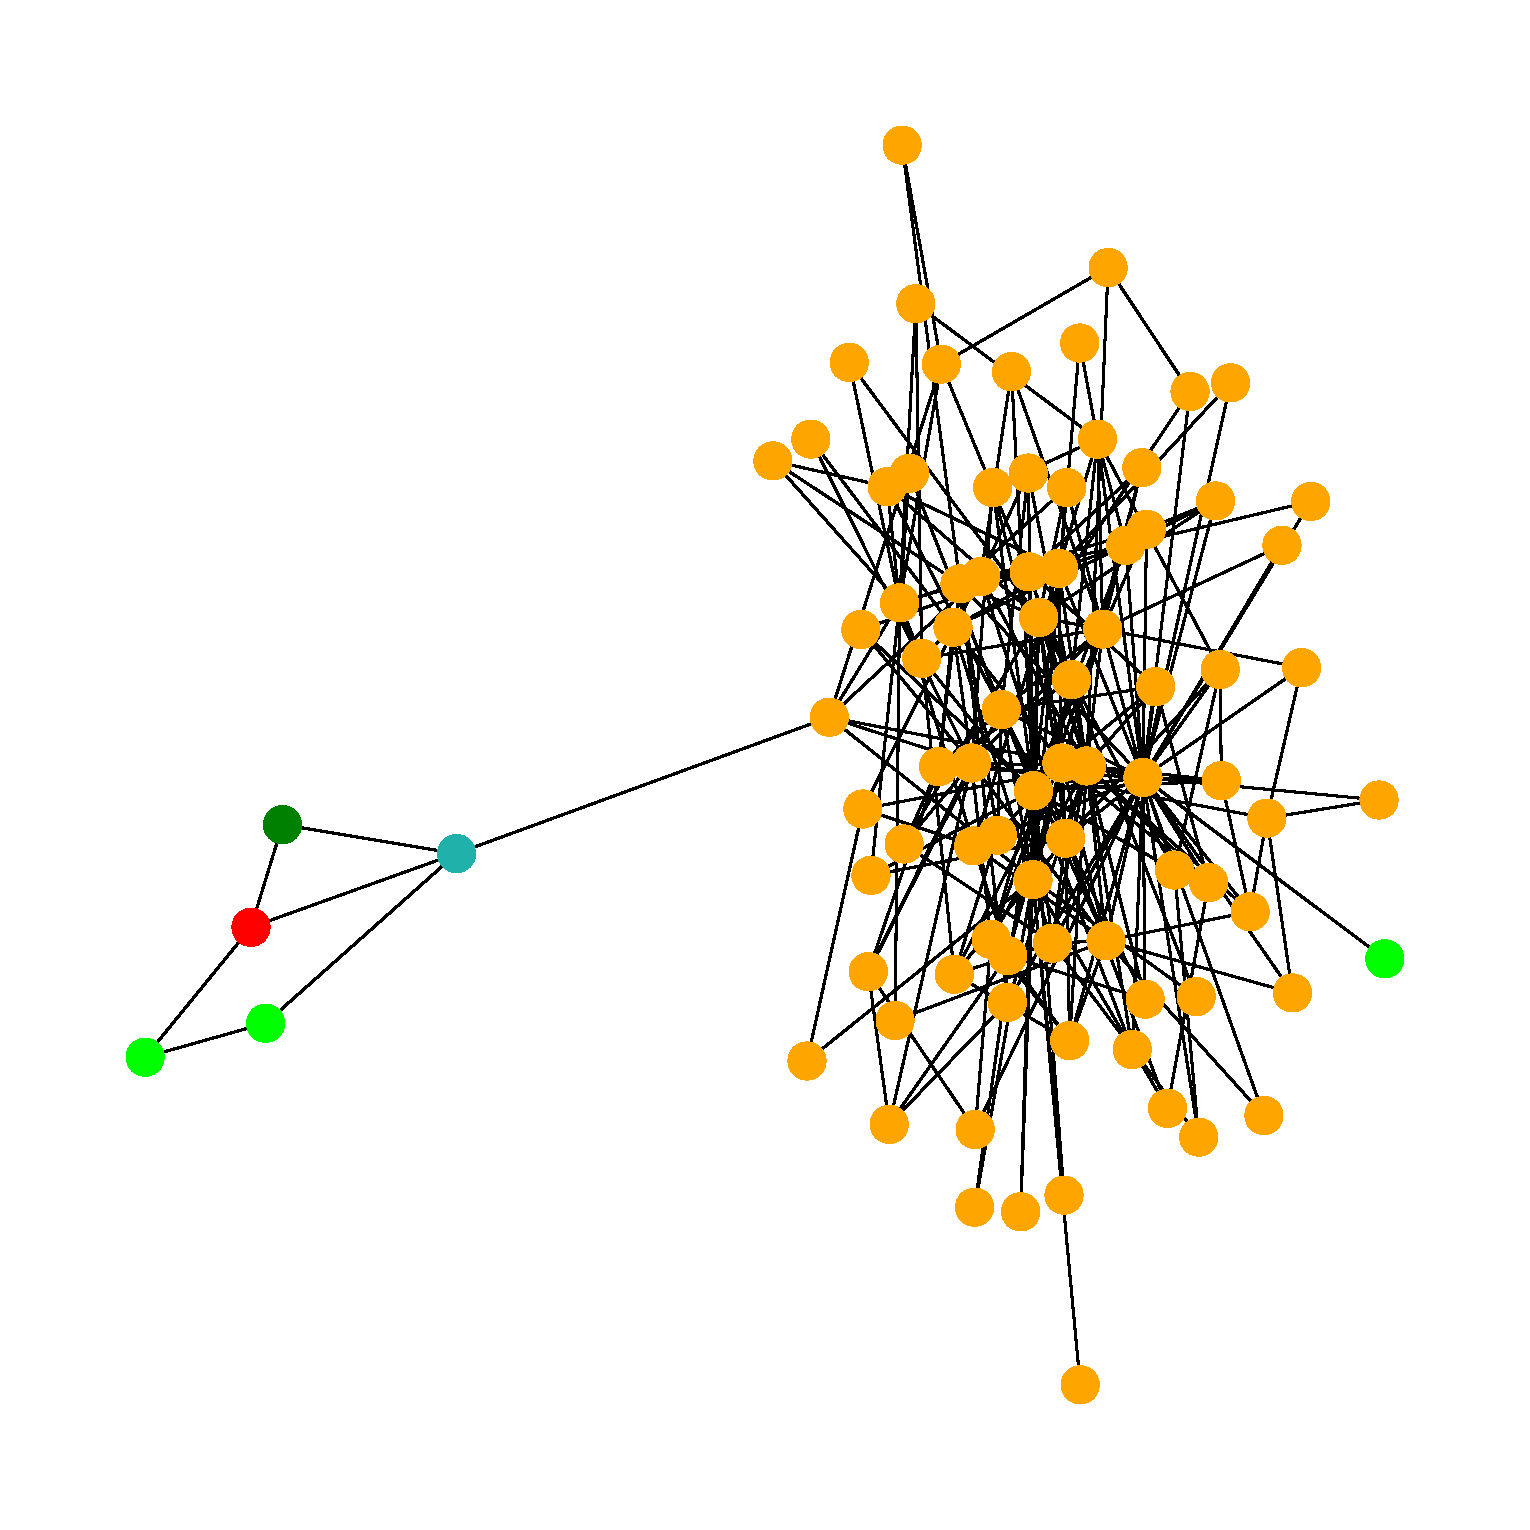
\includegraphics[width=\textwidth]{img/BA-Shapes-VIS-COMP-GRAPH.pdf}
        \caption{BA-Shapes}
    \end{subfigure}
    \hfill
    \begin{subfigure}[b]{0.4\textwidth}
        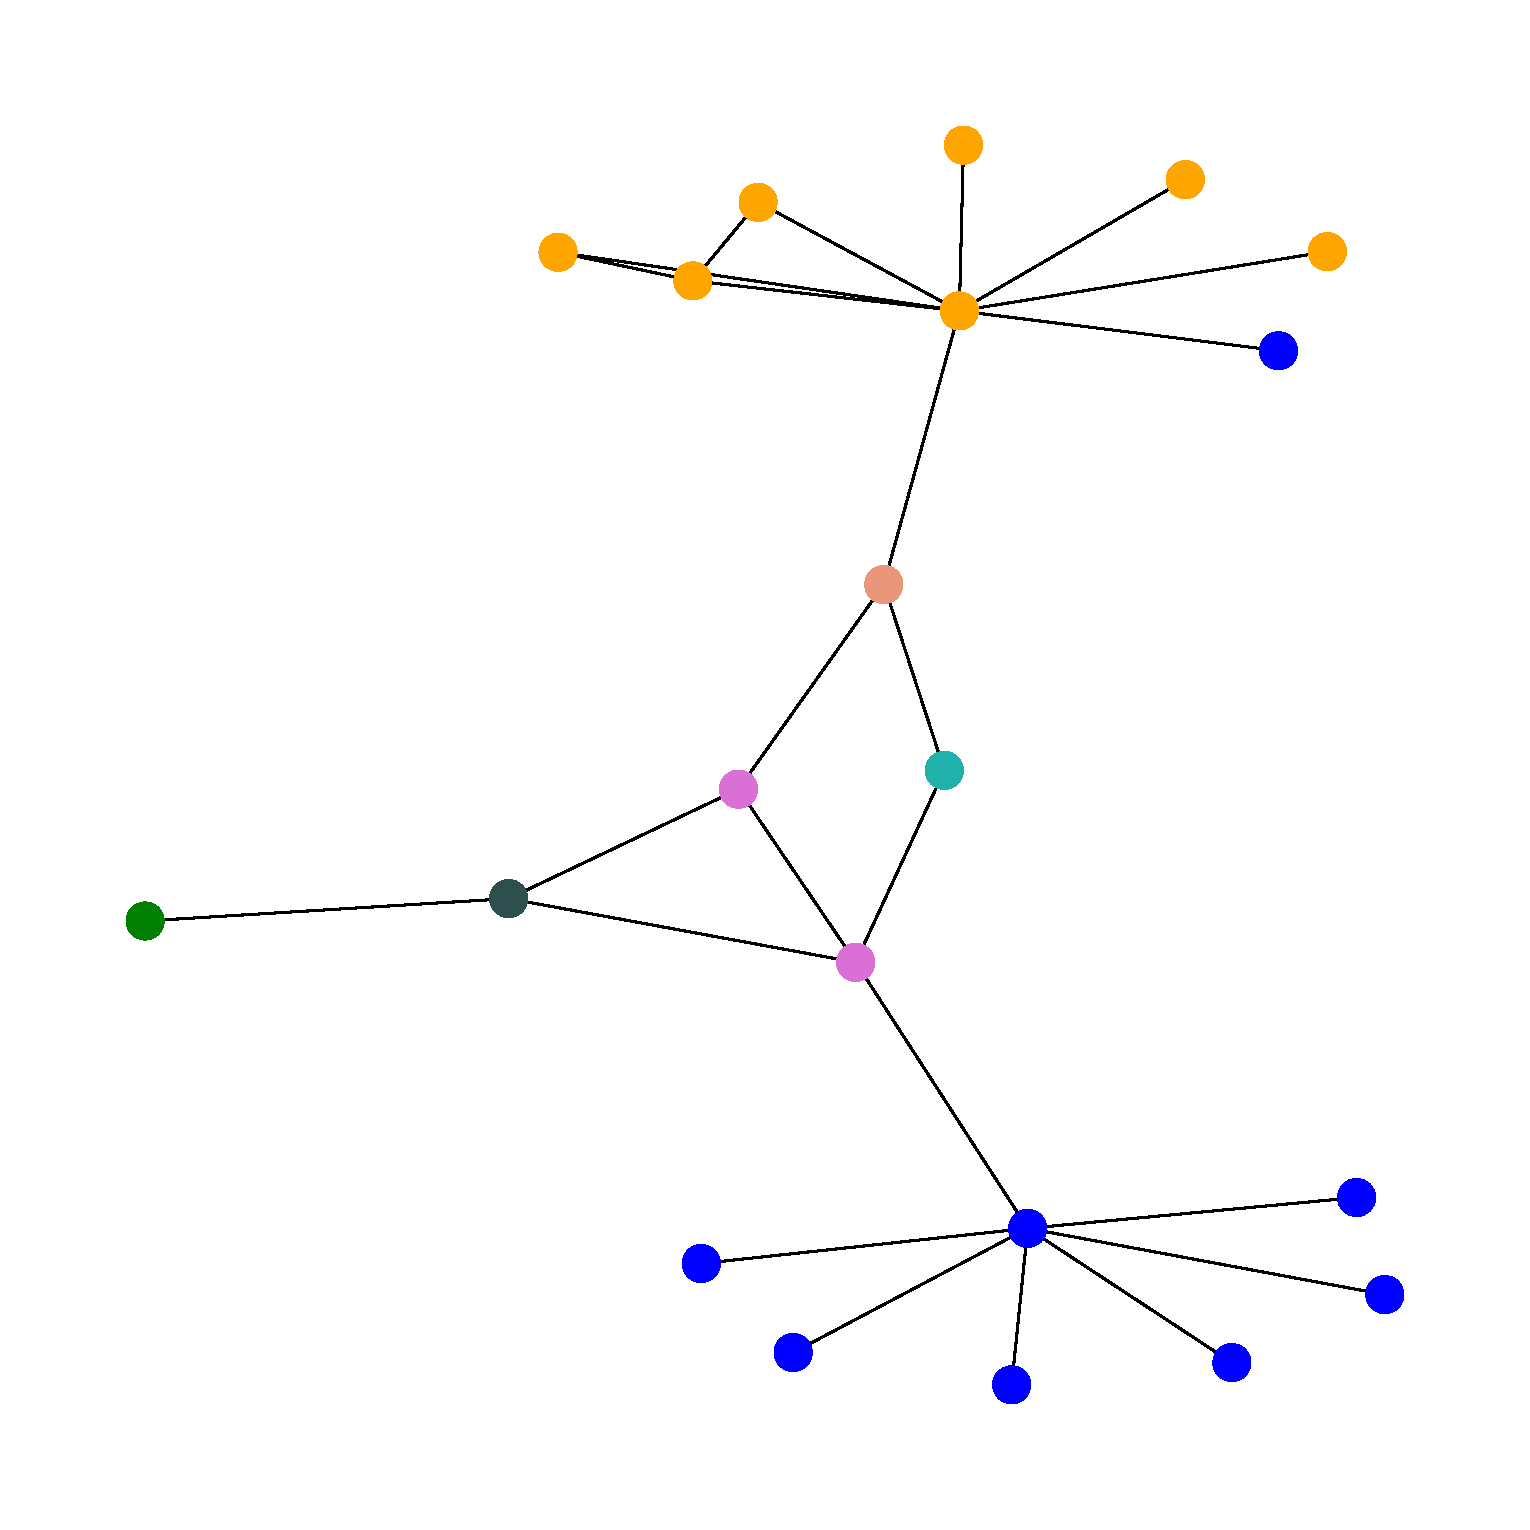
\includegraphics[width=\textwidth]{img/BA-Community-VIS-COMP-GRAPH.pdf}
        \caption{BA-Community}
    \end{subfigure}
    
    \vspace{0.5cm}
    
    \begin{subfigure}[b]{0.4\textwidth}
        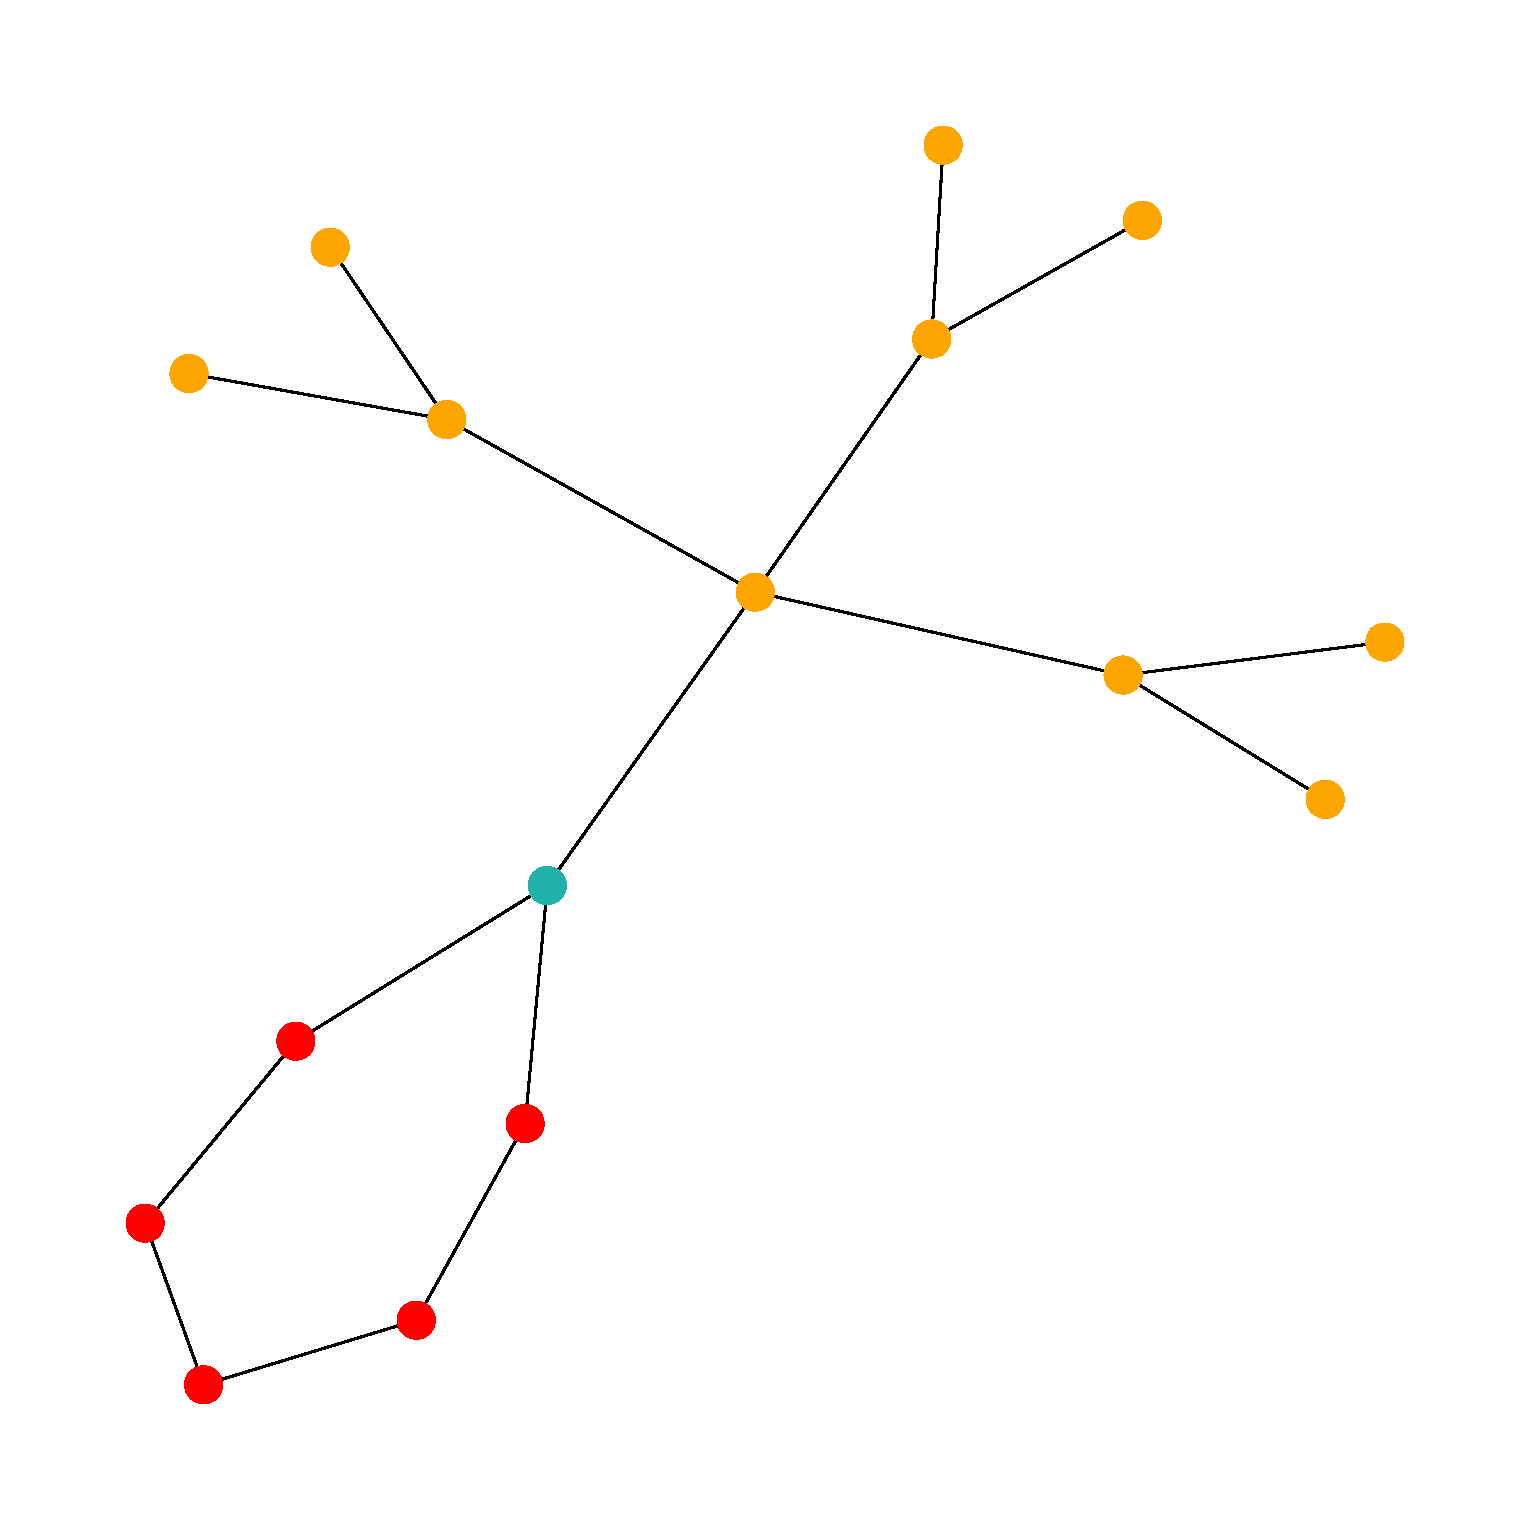
\includegraphics[width=\textwidth]{img/Tree-Cycles-VIS-COMP-GRAPH.pdf}
        \caption{Tree-Cycles}
    \end{subfigure}
    \hfill
    \begin{subfigure}[b]{0.4\textwidth}
        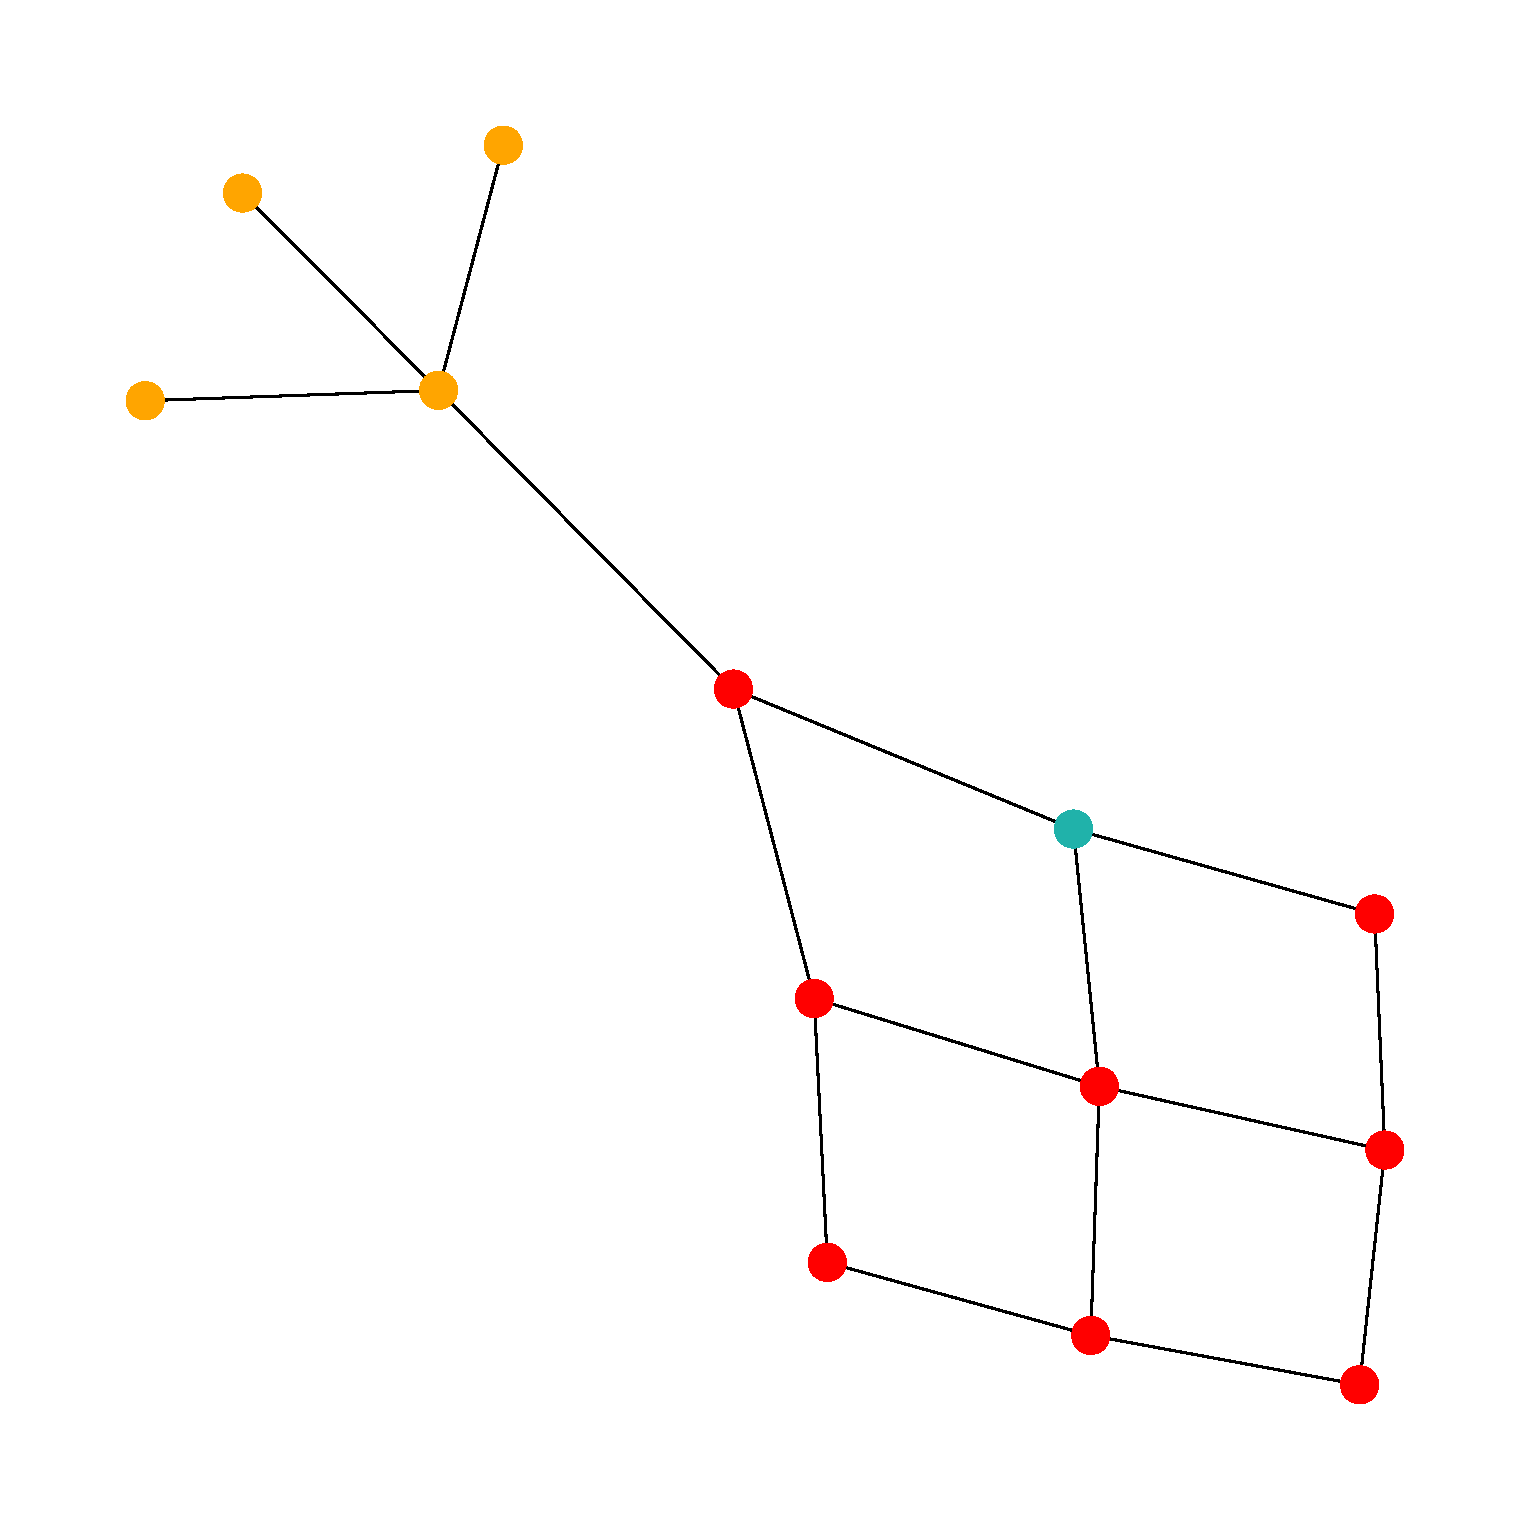
\includegraphics[width=\textwidth]{img/Tree-Grid-VIS-COMP-GRAPH.pdf}
        \caption{Tree-Grid}
    \end{subfigure}
    
    \vspace{0.5cm}
    
    \begin{subfigure}[b]{0.4\textwidth}
        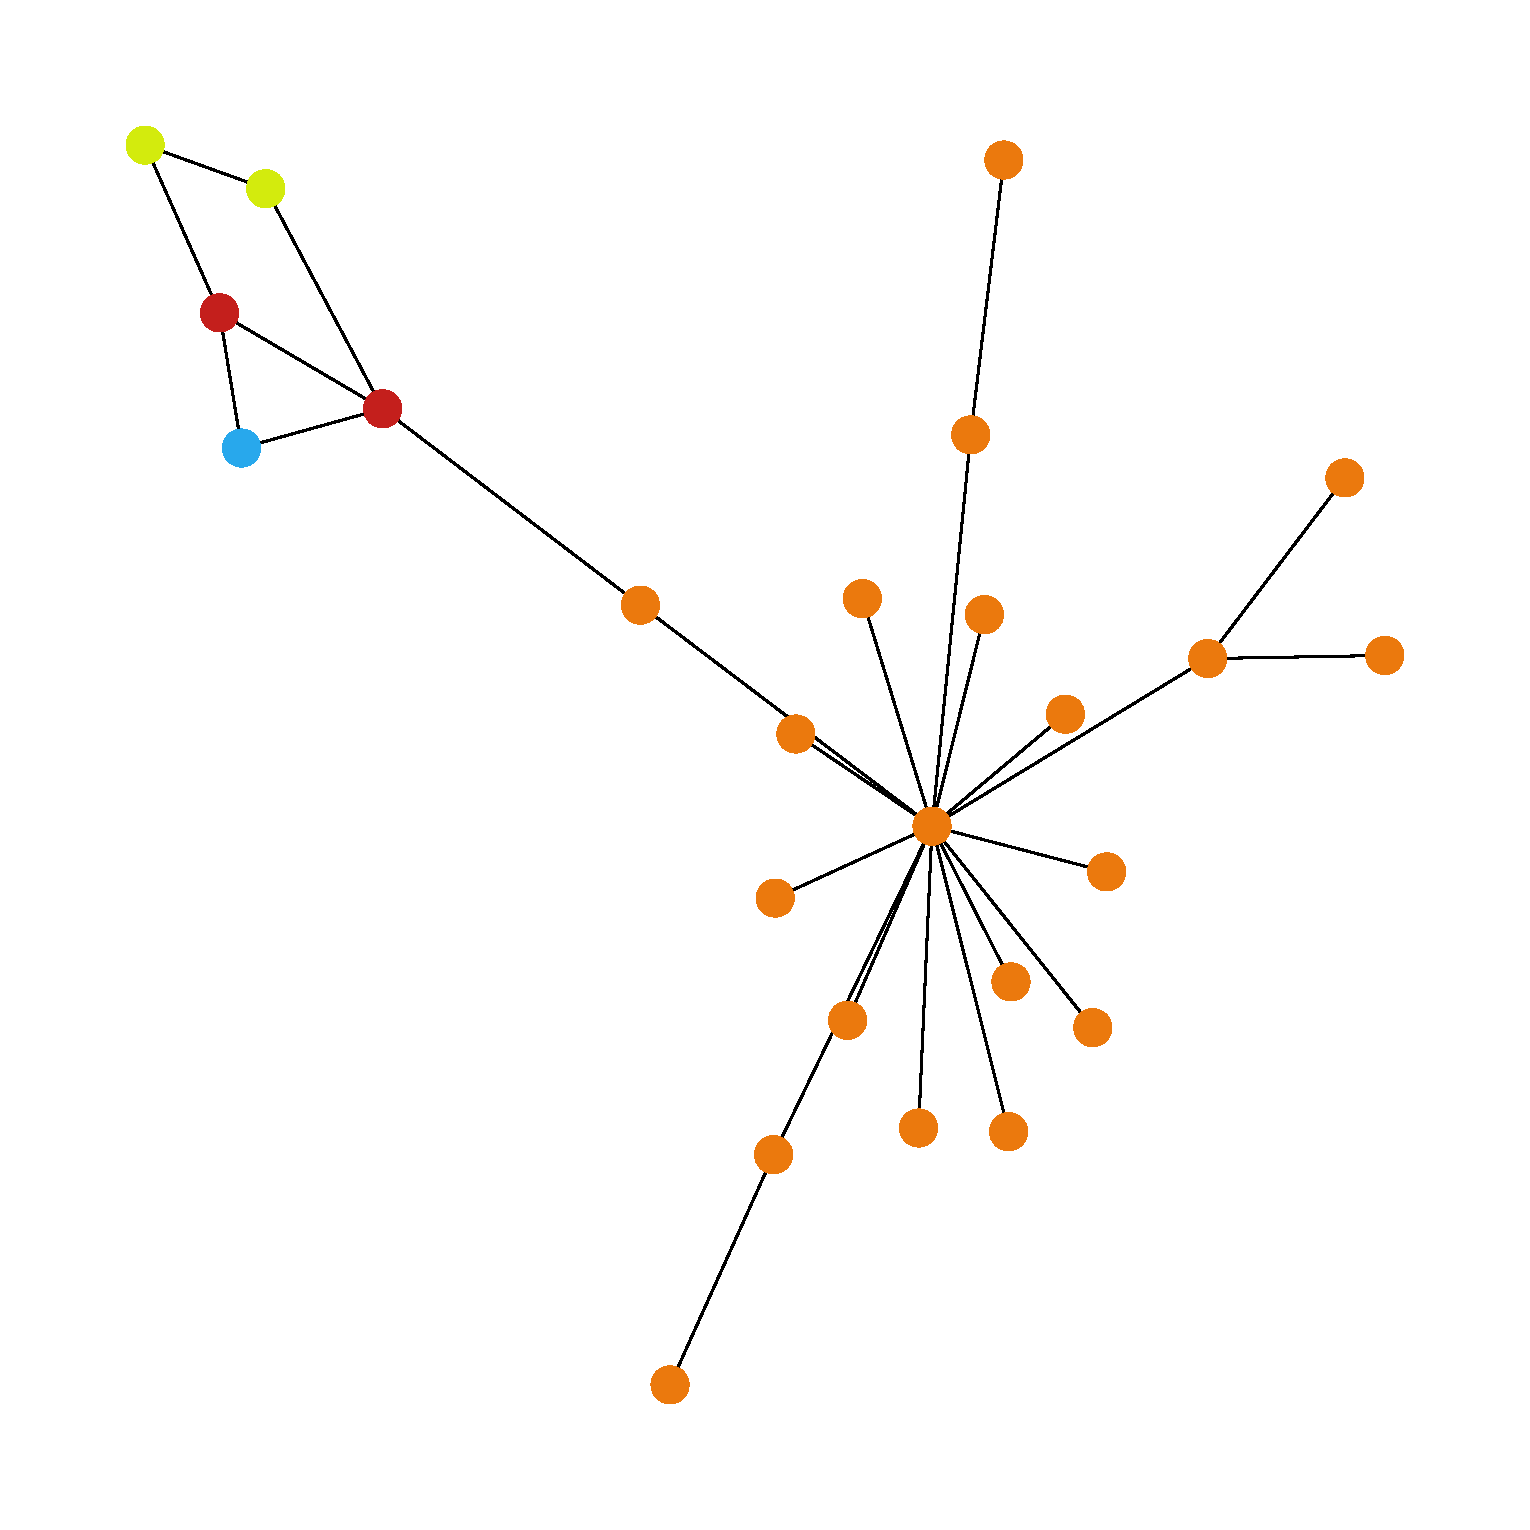
\includegraphics[width=\textwidth]{img/BA-2Motif-VIS-UNLABELED.pdf}
        \caption{BA-2Motif}
    \end{subfigure}
    \hfill
    \begin{subfigure}[b]{0.4\textwidth}
        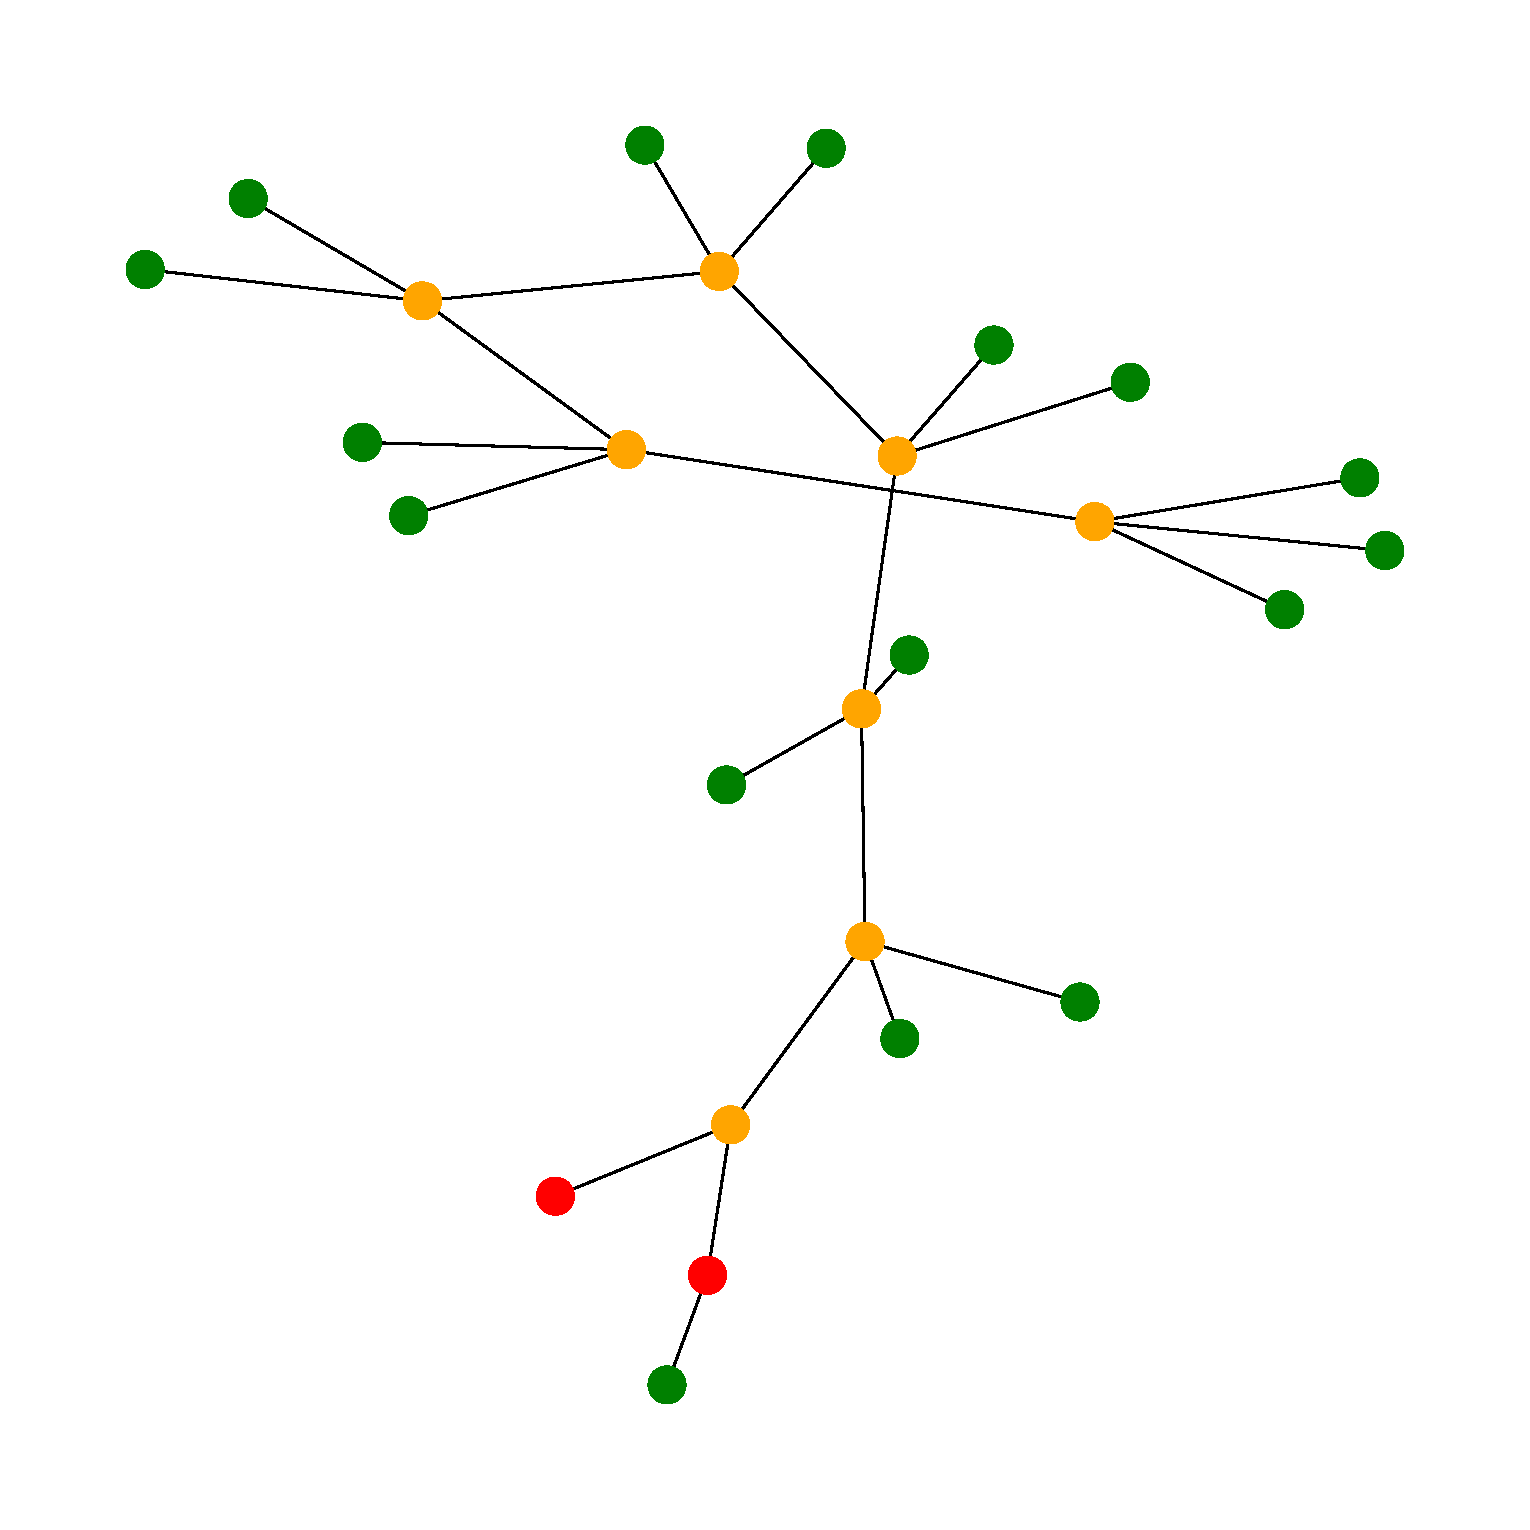
\includegraphics[width=\textwidth]{img/MUTAG-VIS-LARGE-UNLABELED.pdf}
        \caption{MUTAG}
    \end{subfigure}

    \caption[Visualization of original PGExplainer datasets]{Visualization of all six datasets. For node datasets (a-d) the target prediction node where the computational graph is computed from is colored in light blue.}
\end{figure}

\section{Replication Hyperparameter Searches}
\label{sec:sweeps}
The following tables contain the grid search configurations for the explainer on each target model. The first row includes the configuration used in the original codebase \cite{luo2020parameterized} and the second row contains the configurations used in \cite{holdijk2021re}. For BA-Community (see Table \ref{tab:BA-Community_sweep}) both configurations are identical, and the second row is thus omitted. The last section of each table contains the set of the values that we tested for each parameter. The optimal settings for our explainer implementation are highlighted in each column. Note that we optimize Tree-Cycles (see Table \ref{tab:Tree-Cycles_sweep}) and BA-2Motif (see Table \ref{tab:BA-2M-sweep}) towards a minimal metric score, as discussed in Section \ref{sec:ind_results}.

\newcolumntype{Y}{>{\centering\arraybackslash}X}
\begin{table}[h]
  \centering
  \scriptsize
  \begin{tabular}{|c|c|c|c|c|c|c|c|c|c|}
  \hline
  \multicolumn{10}{|c|}{\textbf{BA-Shapes}} \\ \hline
  $a$ & $K$ & $b$ & $E$ & $\eta$ & $S$ & $\alpha_e$ & $\alpha_s$ & $\tau_0$ & $\tau_T$ \\ \hline
  $N$ & 1 & 0.0 & 10 & 0.003 & - & 1.0 & 0.05 & 1.0 & 0.05 \\ \hline
  $N$ & 1 & 0.0 & 10 & 0.003 & - & 1.0 & 0.05 & 5.0 & 2.0 \\ \hline
  5 & \textbf{1} & 0.0 & 10 & 0.0003 & 74 & \textbf{0.1} & 0.005 & 5.0 & \textbf{1} \\
   & 5 &  &  & \textbf{0.003} & 75 & 0.5 & \textbf{0.05} &  & 2 \\
   & 10 &  &  & 0.03 & 76 & 1.0 & 0.1 &  & 5 \\ \hline
  \end{tabular}
  \caption[BA-Shapes grid search]{First two rows show hyperparameter settings used in \cite{luo2020parameterized} and \cite{holdijk2021re}, respectively. Last section contains our grid search configuration. Bolded values indicate the best performance.}
\end{table}

\begin{table}[h]
  \centering
  \scriptsize
  \begin{tabular}{|c|c|c|c|c|c|c|c|c|c|}
  \hline
  \multicolumn{10}{|c|}{\textbf{BA-Community}} \\ \hline
  $a$ & $K$ & $b$ & $E$ & $\eta$ & $S$ & $\alpha_e$ & $\alpha_s$ & $\tau_0$ & $\tau_T$ \\ \hline
  $N$ & 1 & 0.5 & 20 & 0.003 & - & 1.0 & 0.05 & 1.0 & 1.0 \\ \hline
  64 & 1 & \textbf{0.0} & 20 & \textbf{0.003} & 74 & \textbf{1.0} & 0.05 & 1.0 & 1.0 \\
   & \textbf{5} & 0.5 &  & 0.0003 & 75 & 0.1 & \textbf{0.1} &  & \textbf{5.0} \\
   & 10 &  &  &  & 76 &  &  &  &  \\ \hline
  \end{tabular}
  \caption[BA-Community grid search]{First row shows hyperparameter settings used in \cite{luo2020parameterized} and \cite{holdijk2021re}. Last section contains our grid search configuration. Bolded values indicate the best performance.}
  \label{tab:BA-Community_sweep}
\end{table}

\begin{table}[h]
  \centering
  \scriptsize
  \begin{tabular}{|c|c|c|c|c|c|c|c|c|c|}
  \hline
  \multicolumn{10}{|c|}{\textbf{Tree-Cycles}} \\ \hline
  $a$ & $K$ & $b$ & $E$ & $\eta$ & $S$ & $\alpha_e$ & $\alpha_s$ & $\tau_0$ & $\tau_T$ \\ \hline
  $N$ & 1 & 0.0 & 20 & 0.003 & - & 0.01 & 0.0001 & 5.0 & 5.0 \\ \hline
  $N$ & 1 & 0.0 & 20 & 0.003 & - & 10.0 & 0.1 & 1.0 & 5.0 \\ \midrule
  5 & 1 & 0.0 & 20 & \textbf{0.0003} & 74 & 0.01 & \textbf{0.0001} & 1.0 & \textbf{1.0} \\
   & \textbf{5} &  &  & 0.003 & 75 & \textbf{1.0} & 0.05 &  & 5.0 \\
   & 10 &  &  &  & 76 & 10.0 & 0.1 &  &  \\ \hline
  \end{tabular}
  \caption[Tree-Cycles grid search]{First two rows show hyperparameter settings used in \cite{luo2020parameterized} and \cite{holdijk2021re}, respectively. Last section contains our grid search configuration. Bolded values indicate the best performance.}
  \label{tab:Tree-Cycles_sweep}
\end{table}

\begin{table}[h]
  \centering
  \scriptsize
  \begin{tabular}{|c|c|c|c|c|c|c|c|c|c|}
  \hline
  \multicolumn{10}{|c|}{\textbf{Tree-Grid}} \\ \hline
  $a$ & $K$ & $b$ & $E$ & $\eta$ & $S$ & $\alpha_e$ & $\alpha_s$ & $\tau_0$ & $\tau_T$ \\ \hline
  $N$ & 1 & 0.0 & 30 & 0.01 & - & 1.0 & 0.01 & 5.0 & 5.0 \\ \hline
  $N$ & 1 & 0.0 & 30 & 0.003 & - & 1.0 & 1.0 & 5.0 & 2.0 \\ \midrule
  24 & 1 & 0.0 & 30 & 0.0003 & 74 & 0.1 & 0.01 & 5.0 & \textbf{2.0} \\
   & \textbf{5} &  & 30 & \textbf{0.003} & 75 & \textbf{1.0} & \textbf{0.5} &  & 5.0 \\
   & 10 &  & 30 & 0.01 & 76 & 10 & 1.0 &  &  \\ 
   &  &  &  & 0.05 &  &  &  &  &  \\ \hline
  \end{tabular}
  \caption[Tree-Grid grid search]{First two rows show hyperparameter settings used in \cite{luo2020parameterized} and \cite{holdijk2021re}, respectively. Last section contains our grid search configuration. Bolded values indicate the best performance.}
\end{table}

\begin{table}[h]
  \centering
  \scriptsize
  \begin{tabular}{|c|c|c|c|c|c|c|c|c|c|}
  \hline
  \multicolumn{10}{|c|}{\textbf{BA-2Motif}} \\ \hline
  $a$ & $K$ & $b$ & $E$ & $\eta$ & $S$ & $\alpha_e$ & $\alpha_s$ & $\tau_0$ & $\tau_T$ \\ \hline
  $N$ & 1 & 0.0 & 10 & 0.003 & - & 0.0 & 0.00 & 1.0 & 0.0 \\ \hline
  $N$ & 1 & 0.0 & 20 & 0.005 & - & 0.01 & 0.03 & 5.0 & 1.0 \\ \midrule
  30 & 1 & 0.0 & 10 & 0.0003 & 74 & 0.01 & 0.03 & 5.0 & \textbf{1.0} \\
   & 5 &  & \textbf{20} & 0.003 & 75 & \textbf{0.1} &  &  & 5.0 \\
   & \textbf{10} &  &  & 0.005 & 76 &  &  &  &  \\
   &  &  &  & \textbf{0.01} &  &  &  &  &  \\ \hline
  \end{tabular}
  \caption[BA-2Motif grid search]{First two rows show hyperparameter settings used in \cite{luo2020parameterized} and \cite{holdijk2021re}, respectively. Last section contains our grid search configuration. Bolded values indicate the best performance.}
  \label{tab:BA-2M-sweep}
\end{table}

\begin{table}[h]
  \centering
  \scriptsize
  \begin{tabular}{|c|c|c|c|c|c|c|c|c|c|}
  \hline
  \multicolumn{10}{|c|}{\textbf{MUTAG}} \\ \hline
  $a$ & $K$ & $b$ & $E$ & $\eta$ & $S$ & $\alpha_e$ & $\alpha_s$ & $\tau_0$ & $\tau_T$ \\ \hline
  $N$ & 1 & 0.0 & 10 & 0.01 & - & 1.0 & 0.01 & 5.0 & 5.0 \\ \hline
  $N$ & 1 & 0.0 & 30 & 0.0003 & - & 1.0 & 0.005 & 5.0 & 5.0 \\ \midrule
  30 & 1 & 0.0 & 10 & 0.0003 & 74 & 0.1 & 0.01 & 5.0 & \textbf{1.0} \\
   & 5 &  & \textbf{20} & 0.003 & 75 & \textbf{1.0} & \textbf{0.005} &  & 5.0 \\
   & \textbf{10} &  & 30 & \textbf{0.01} & 76 &  &  &  &  \\ \hline
  \end{tabular}
  \caption[MUTAG grid search]{First two rows show hyperparameter settings used in \cite{luo2020parameterized} and \cite{holdijk2021re}, respectively. Last section contains our grid search configuration. Bolded values indicate the best performance.}
\end{table}

\clearpage
\section{Multiple Explanation Visualizations}
\label{sec:grid_vis}
The following figures \ref{fig:grid-BA-Shapes-explanations}, \ref{fig:grid-BA-Community-explanations}, \ref{fig:grid-Tree-Cycles-explanations}, \ref{fig:grid-Tree-Grid-explanations}, \ref{fig:grid-BA-2Motif-explanations}, \ref{fig:grid-MUTAG-explanations} contain 16 randomly sampled explanations for the best explainer model of every dataset. For graph tasks all nodes of the input graph are included, while for node tasks only the nodes of the local computation graph from the prediction motif node are shown.

% REMOVE draw=black TO REMOVE EDGES
\begin{figure}[htbp]
    \centering
    \begin{tikzpicture}
      % 4x4 grid: row = 0 to 3, col = 0 to 3
      \foreach \row in {0,...,3} {
        \foreach \col in {0,...,3} {
          \pgfmathtruncatemacro{\num}{\col + 4 * \row}
          \node[draw=black, thin, inner sep=0pt] at (\col*4, -\row*4)
            {\includegraphics[width=3.5cm]{img/BA-Shapes/graph_\num_explanation.pdf}};
        }
      }
    \end{tikzpicture}
    \caption{Grid of BA-Shapes explanations (top-6 edges)}
    \label{fig:grid-BA-Shapes-explanations}
\end{figure}

\begin{figure}[htbp]
    \centering
    \begin{tikzpicture}
      % 4x4 grid: row = 0 to 3, col = 0 to 3
      \foreach \row in {0,...,3} {
        \foreach \col in {0,...,3} {
          \pgfmathtruncatemacro{\num}{\col + 4 * \row}
          \node[draw=black, thin, inner sep=0pt] at (\col*4, -\row*4)
            {\includegraphics[width=3.5cm]{img/BA-Community/graph_\num_explanation.pdf}};
        }
      }
    \end{tikzpicture}
    \caption{Grid of BA-Community explanations (top-6 edges)}
    \label{fig:grid-BA-Community-explanations}
\end{figure}

\begin{figure}[htbp]
    \centering
    \begin{tikzpicture}
      % 4x4 grid: row = 0 to 3, col = 0 to 3
      \foreach \row in {0,...,3} {
        \foreach \col in {0,...,3} {
          \pgfmathtruncatemacro{\num}{\col + 4 * \row}
          \node[draw=black, thin, inner sep=0pt] at (\col*4, -\row*4)
            {\includegraphics[width=3.5cm]{img/Tree-Cycles/graph_\num_explanation.pdf}};
        }
      }
    \end{tikzpicture}
    \caption{Grid of Tree-Cycles explanations (top-6 edges)}
    \label{fig:grid-Tree-Cycles-explanations}
\end{figure}

\begin{figure}[htbp]
    \centering
    \begin{tikzpicture}
      % 4x4 grid: row = 0 to 3, col = 0 to 3
      \foreach \row in {0,...,3} {
        \foreach \col in {0,...,3} {
          \pgfmathtruncatemacro{\num}{\col + 4 * \row}
          \node[draw=black, thin, inner sep=0pt] at (\col*4, -\row*4)
            {\includegraphics[width=3.5cm]{img/Tree-Grid/graph_\num_explanation.pdf}};
        }
      }
    \end{tikzpicture}
    \caption{Grid of Tree-Grid explanations (top-12 edges)}
    \label{fig:grid-Tree-Grid-explanations}
\end{figure}

\begin{figure}[htbp]
    \centering
    \begin{tikzpicture}
      % 4x4 grid: row = 0 to 3, col = 0 to 3
      \foreach \row in {0,...,3} {
        \foreach \col in {0,...,3} {
          \pgfmathtruncatemacro{\num}{\col + 4 * \row}
          \node[draw=black, thin, inner sep=0pt] at (\col*4, -\row*4)
            {\includegraphics[width=3.5cm]{img/BA-2Motif/graph_\num_explanation.pdf}};
        }
      }
    \end{tikzpicture}
    \caption{Grid of BA-2Motif explanations (top-5 edges)}
    \label{fig:grid-BA-2Motif-explanations}
\end{figure}

\begin{figure}[htbp]
    \centering
    \begin{tikzpicture}
      % 4x4 grid: row = 0 to 3, col = 0 to 3
      \foreach \row in {0,...,3} {
        \foreach \col in {0,...,3} {
          \pgfmathtruncatemacro{\num}{\col + 4 * \row}
          \node[draw=black, thin, inner sep=0pt] at (\col*4, -\row*4)
            {\includegraphics[width=3.5cm]{img/MUTAG/graph_\num_explanation.pdf}};
        }
      }
    \end{tikzpicture}
    \caption{Grid of MUTAG explanations (top-10 edges)}
    \label{fig:grid-MUTAG-explanations}
\end{figure}

\clearpage
\section{NeuroSAT explainer Hyperparameter Searches}
\label{sec:neurSAT_sweeps}

The following tables contain the grid search configurations for the NeuroSAT explainer models with either the soft constraint (see Table \ref{tab:sweep_conf_soft}) or the hard constraint (see Table \ref{tab:sweep_conf_hard}) applied. The columns contain the values tested for the corresponding hyperparameter. The optimal settings for each explainer implementation are highlighted. Figure \ref{fig:soft-sweep} shows the AUROC range of all runs performed in the grid search for the soft constraint explainer.

\begin{table}[h]
  \centering
  \scriptsize
  \begin{tabular}{|c|c|c|c|c|c|c|c|c|c|c|c|c|}
  \hline
  \multicolumn{11}{|c|}{\textbf{Soft Constraint Explainer}} \\ \hline
  $K$ & $E$ & $\eta$ & $S$ & $\alpha_e$ & $\alpha_s$ & $\tau_0$ & $\tau_T$ & $\alpha_{concat}$ & $\alpha_C$ & $\alpha_{AdamW}$ \\ \hline
  1 & \textbf{20} & \textbf{0.0003} & 75 & 0.1 & \textbf{0.001} & 5.0 & \textbf{1.0} & False & 0.1 & False\\ 
  \textbf{5} & 30 & 0.003 & 76 & \textbf{1.0} & 0.01 &  & 5.0 & \textbf{True} & 1.0 & \textbf{True}\\ 
   & 50 & 0.01 &  &  & 0.1 &  &  &  & \textbf{10.0} & \\ \hline
  \end{tabular}
  \caption[NeuroSAT soft constraint grid search]{Grid search results over hyperparameter space for the NeuroSAT explainer that uses a soft constraint. Bolded values indicate the best performance.}
  \label{tab:sweep_conf_soft}
\end{table}

\begin{table}[h]
    \centering
    \scriptsize
    \begin{tabular}{|c|c|c|c|c|c|c|c|c|c|c|}
    \hline
    \multicolumn{10}{|c|}{\textbf{Hard Constraint Explainer}} \\ \hline
    $K$ & $E$ & $\eta$ & $S$ & $\alpha_e$ & $\alpha_s$ & $\tau_0$ & $\tau_T$ & $\alpha_{concat}$ & $\alpha_{arch}$ \\ \hline
    1 & 20 & \textbf{0.00003} & 75 & 0.1 & \textbf{0.01} & 5.0 & \textbf{1.0} & \textbf{False} & False \\
    \textbf{5} & 30 & 0.0003 & 76 & \textbf{1.0} & 0.1 &  & 5.0 & True & \textbf{True} \\
     & \textbf{50} & 0.003 &  &  & 1.0 &  &  &  & \\
     &  & 0.01 &  &  &  &  &  &  & \\ \hline
    \end{tabular}
    \caption[NeuroSAT hard constraint grid search]{Grid search results over hyperparameter space for the NeuroSAT explainer that uses a hard constraint. Bolded values indicate the best performance.}
    \label{tab:sweep_conf_hard}
\end{table}

\begin{figure}
  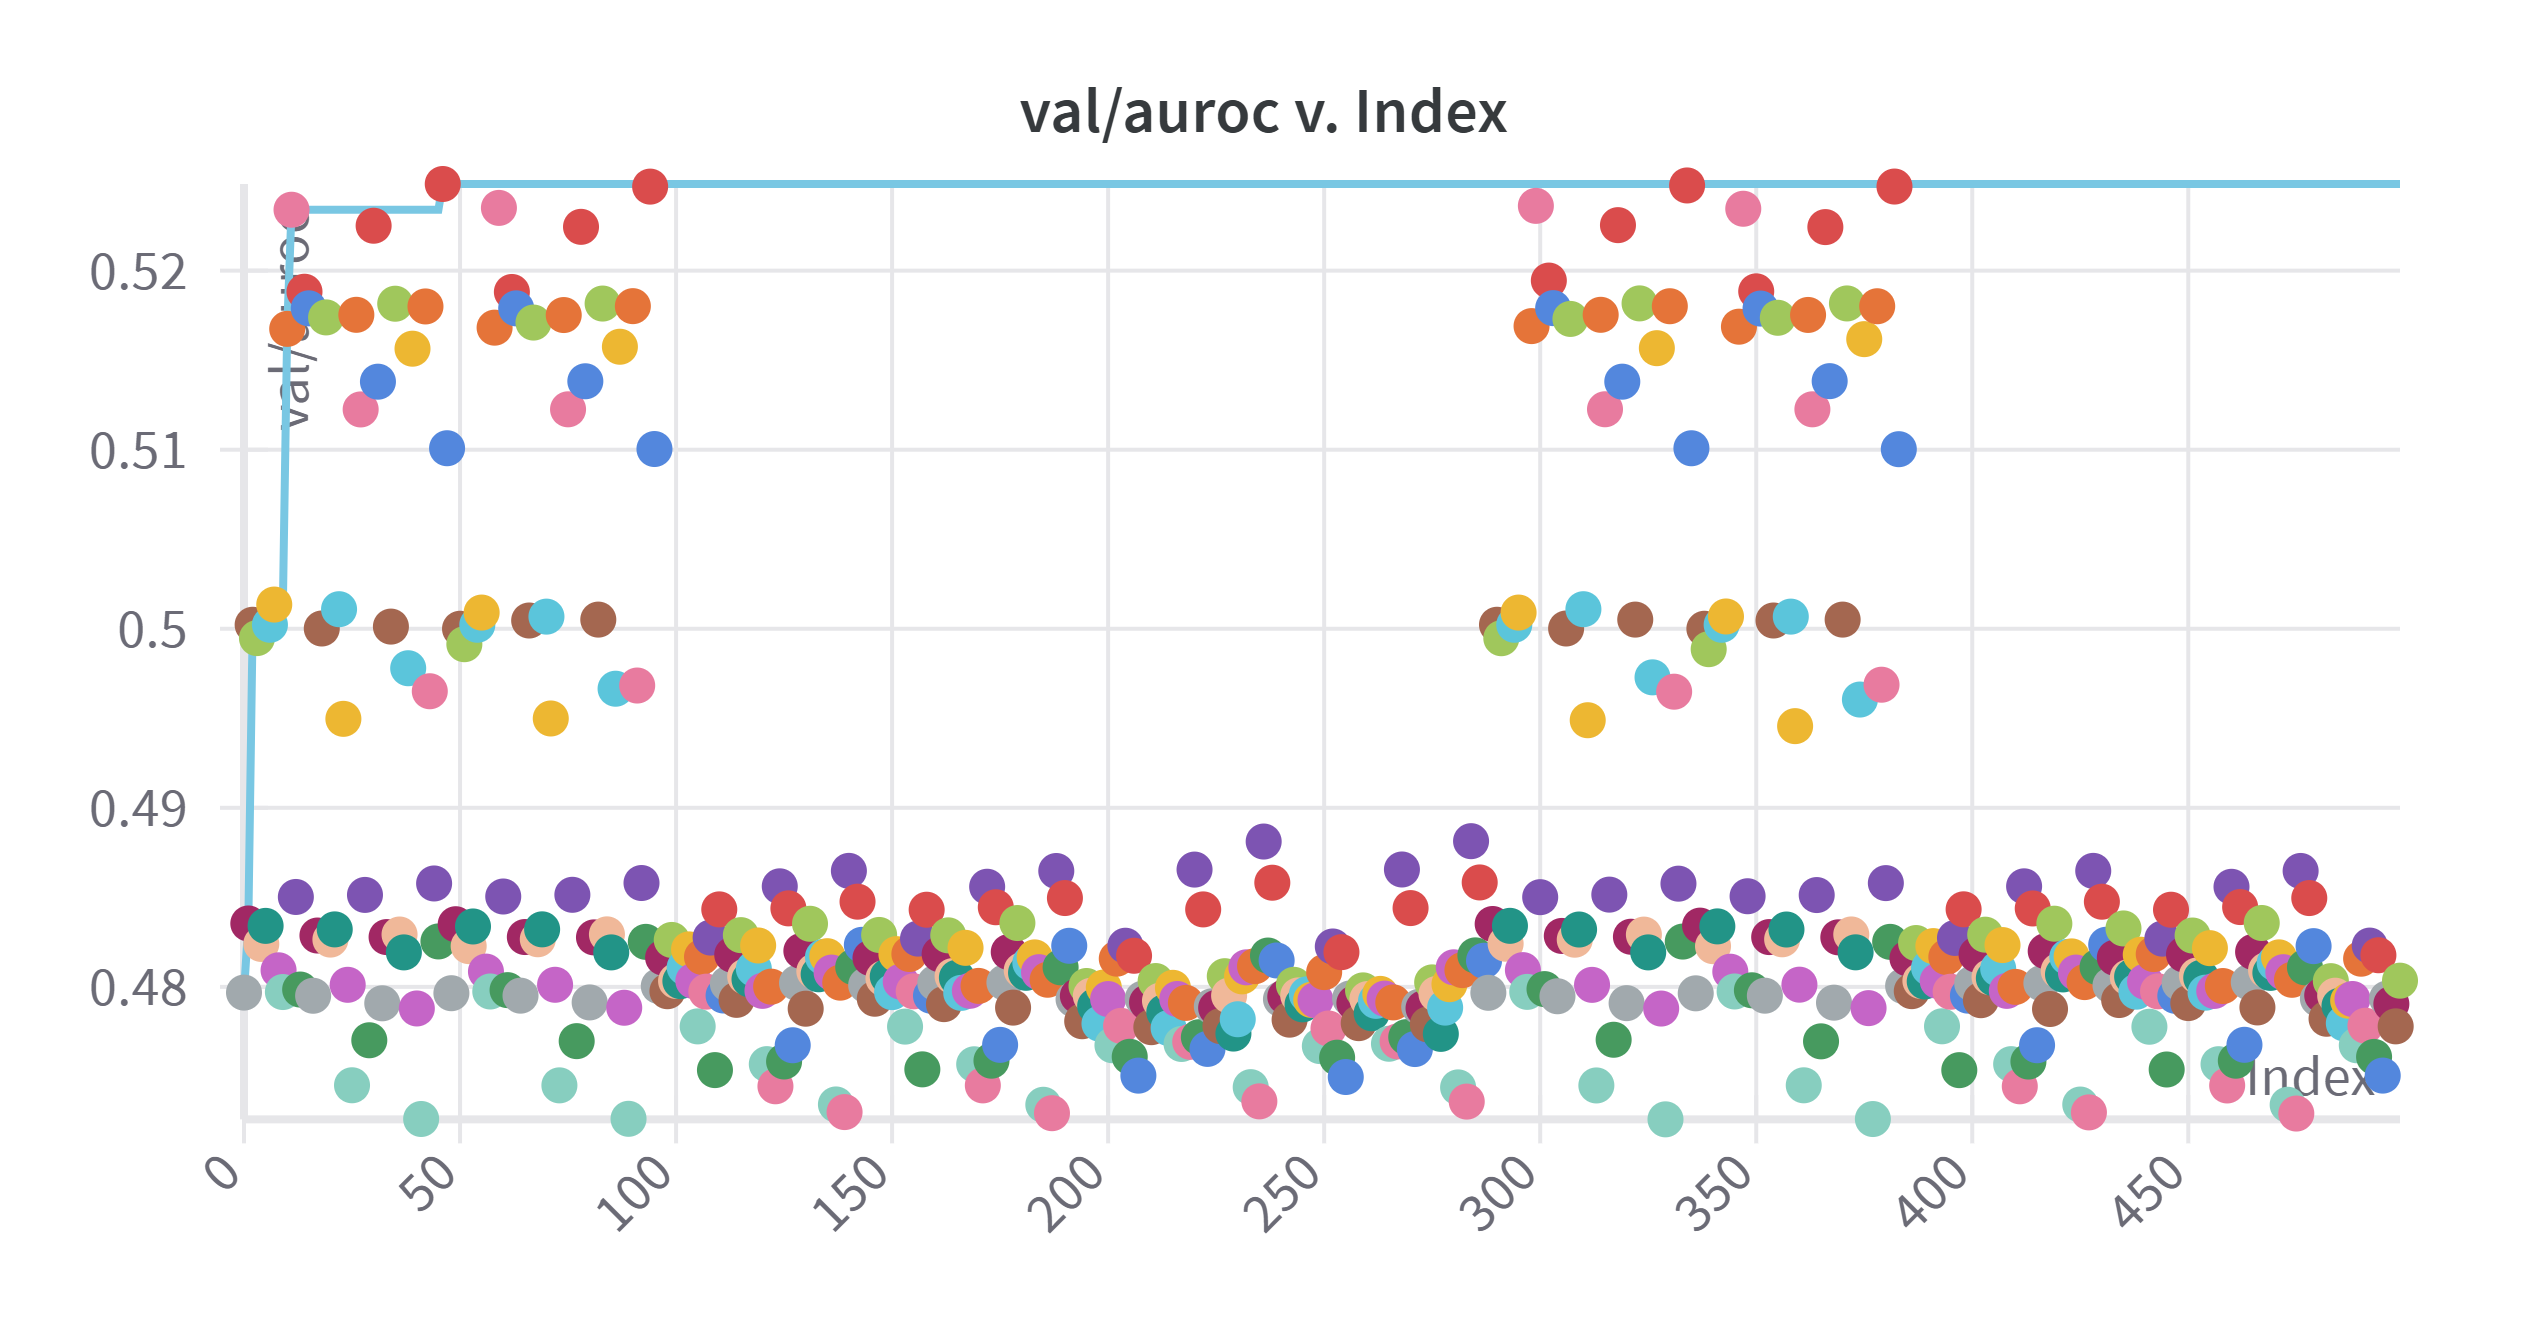
\includegraphics[width=\linewidth]{img/NeuroSAT-soft_sweep.png}
  \caption[Grid search results of soft constraint explainer]{Grid search results of all runs on the soft constraint explainer using WandB \cite{wandb}.}
  \label{fig:soft-sweep}
\end{figure}

\section{Satisfiability of a Hard Constraint Explanation}
\label{sec:sat_expl_hard_cons}
The SAT formula represented by the top-$k$ edges of the validation problem that achieved the highest individual AUROC score for the seed 0 run, with $k$ being the number of edges in its corresponding MUS, is defined as:
\begin{align*}
& (174 \lor 175 \lor 173 \lor 169) \land \\
& (171 \lor 170 \lor 173) \land \\
& (171 \lor 175 \lor 168 \lor 173) \land \\
& (172 \lor 174 \lor 171) \land \\
& (171 \lor 169 \lor 168 \lor 174) \land \\
& (\neg 170) \land \\
& (170 \lor 173 \lor 168) \land \\
& (\neg 168 \lor 171) \land \\
& (172 \lor \neg 168 \lor \neg 170) \land \\
& (169 \lor 171 \lor 172 \lor \neg 174) \land \\
& (175 \lor 173 \lor 168)
\end{align*}
We note that this subset of clauses is satisfiable and therefore not an unsatisfiable core. It is important to note that setting $k$ as the number of edges in its corresponding MUS only makes sense if the MUS is known to be the \ac{GT}. Since we do not know this, this selection of $k$ can be seen as arbitrary. However, a selection is necessary in the context of PGExplainer, since a dynamic way of getting the most important explanation edges was not provided in the original.